\documentclass{standalone}

\usepackage{tikz}
\usetikzlibrary{patterns}
\usetikzlibrary{patterns.meta}
\usetikzlibrary{arrows.meta}

\begin{document}

	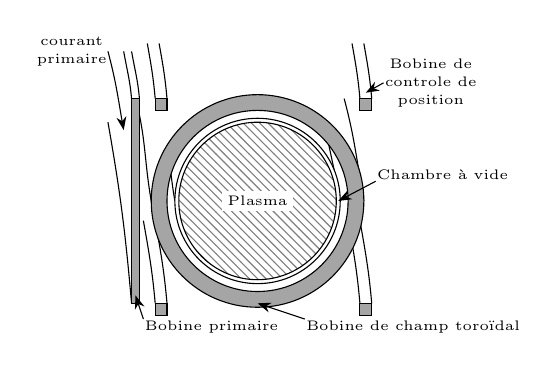
\begin{tikzpicture}

		% plasma
		\draw
	    	(-1.15,0.7)
    		to [out=-80, in=100]
    		(-1.05,0);		
    	\draw
	    	(0.85, 1)
    		to [out=-80, in=100]
    		(1.05,0);		
    	\fill[white] (0,0) circle [radius=1.05cm];
		\draw (0,0) circle [radius=1.05cm];
		
		\fill[pattern=north west lines, pattern color=gray]
    		(0,0) ellipse [x radius=1cm, y radius=1cm];
		\draw (0,0) ellipse [x radius=1cm, y radius=1cm];
		
		% Bobines de controles de la position du bas
		
		\draw
	    	(-1.45,-0.25)
    		to [out=-80, in=95]
    		(-1.3,-1.3);		
    	\draw
	    	(-1.3, -0.25)
    		to [out=-80, in=95]
    		(-1.15,-1.3);
    	\fill[pattern={Lines[angle=-45,distance=0.5pt,line width=0.2pt]}, pattern color=black] (-1.3, -1.3) -- (-1.15,-1.3) -- (-1.15,-1.45) -- (-1.3,-1.45) -- cycle;
    	\draw (-1.3, -1.3) -- (-1.15,-1.3) -- (-1.15,-1.45) -- (-1.3,-1.45) -- cycle;
    	
    	\draw
	    	(1.15,-0.25)
    		to [out=-80, in=95]
    		(1.3,-1.3);		
    	\draw
	    	(1.3, -0.25)
    		to [out=-80, in=95]
    		(1.45,-1.3);
    	\fill[pattern={Lines[angle=-45,distance=0.5pt,line width=0.2pt]}, pattern color=black] (1.45, -1.3) -- (1.3,-1.3) -- (1.3,-1.45) -- (1.45,-1.45) -- cycle;
    	\draw  (1.45, -1.3) -- (1.3,-1.3) -- (1.3,-1.45) -- (1.45,-1.45) -- cycle;
		
		% bobine de champ toroïdal
		\draw
	    	(-1.55,1.3)
    		to [out=-75, in=100]
    		(-1.35,0);		
    	\draw
	    	(1.1, 1.3)
    		to [out=-75, in=100]
    		(1.35,0);
		\fill[white]
			(1.35,0) arc[start angle=0, end angle=360, radius=1.35cm]
			-- (1.15,0) arc[start angle=0, end angle=-360, radius=1.15cm]
			-- cycle;
		\fill[pattern={Lines[angle=-45,distance=0.5pt,line width=0.2pt]}, pattern color=black]
			(1.35,0) arc[start angle=0, end angle=360, radius=1.35cm]
			-- (1.15,0) arc[start angle=0, end angle=-360, radius=1.15cm]
			-- cycle;
			
		\draw (0,0) circle [radius=1.35cm];
		\draw (0,0) circle [radius=1.15cm];
		
		% Bobines de controles de la position du haut
		
		\draw
	    	(-1.4,2)
    		to [out=-80, in=95]
    		(-1.3,1.3);		
    	\draw
	    	(-1.25, 2)
    		to [out=-80, in=95]
    		(-1.15,1.3);
    	\fill[pattern={Lines[angle=-45,distance=0.5pt,line width=0.2pt]}, pattern color=black] (-1.3, 1.3) -- (-1.15,1.3) -- (-1.15,1.15) -- (-1.3,1.15) -- cycle;
    	\draw (-1.3, 1.3) -- (-1.15,1.3) -- (-1.15,1.15) -- (-1.3,1.15) -- cycle;
    	
    	\draw
	    	(1.2,2)
    		to [out=-80, in=95]
    		(1.3,1.3);		
    	\draw
	    	(1.35, 2)
    		to [out=-80, in=95]
    		(1.45,1.3);
    	\fill[pattern={Lines[angle=-45,distance=0.5pt,line width=0.2pt]}, pattern color=black] (1.45, 1.3) -- (1.3,1.3) -- (1.3,1.15) -- (1.45,1.15) -- cycle;
    	\draw  (1.45, 1.3) -- (1.3,1.3) -- (1.3,1.15) -- (1.45,1.15) -- cycle;
    	
    	% bobine primaire
		
		\fill[white] (-1.6, -1.3) -- (-1.6,1.3) -- (-1.5,1.3) -- (-1.5,-1.3) -- cycle;
		\fill[pattern={Lines[angle=-45,distance=0.5pt,line width=0.2pt]}, pattern color=black] (-1.6, -1.3) -- (-1.6,1.3) -- (-1.5,1.3) -- (-1.5,-1.3) -- cycle;
    	\draw (-1.6, -1.3) -- (-1.6,1.3) -- (-1.5,1.3) -- (-1.5,-1.3) -- cycle;
    	
    	\draw
	    	 (-1.9, 1.)
    		to [out=-80, in=95]
    		(-1.6,-1.3);		
    		
    	\draw
	    	 (-1.7, 1.9)
    		to [out=-80, in=95]
    		(-1.6,1.3);		
    		
    	\draw
	    	 (-1.6, 1.9)
    		to [out=-80, in=95]
    		(-1.5,1.3);
    		
    	% Courant primaire
    	
    	\draw[-{Stealth}]
	    	 (-1.9, 1.9)
    		to [out=-75, in=100]
    		(-1.7,0.9);
    		
    	\node[left=-3pt, align=center] at (-1.9, 1.9) {\tiny\shortstack{courant\\ primaire}};
    		
    	% Légende de la figure
    	
    	\draw[{Stealth}-] (1.025,0) -- (1.5,0.25) node[above right=-3pt] {\tiny Chambre à vide};
    	
    	\draw[{Stealth}-] (1.375,1.375) -- (1.6,1.5) node[right=-3pt, align=center] {\tiny\shortstack{Bobine de\\ controle de\\ position}};
    	
    	\draw[{Stealth}-] (0,-1.3) -- (0.6,-1.5) node[below right =-3pt, align=center] {\tiny\shortstack{Bobine de champ toroïdal}};
    	
    	\draw[{Stealth}-] (-1.55,-1.2) -- (-1.45, -1.5) node[below right=-3pt, align=center] {\tiny\shortstack{Bobine primaire}};
    	
    	\node[fill=white, text=black, inner sep=2pt] at (0,0) {\tiny Plasma};
    	
	\end{tikzpicture}

\end{document}